\Section{Analysis- Strategy and Setup}
\label{ch:analysis_strategy}

In this chapter, an overview of the analysis- strategy and setup will be given with a special focus on the physical observable used as the condition for the cINN inference.

\Subsection{Analysis Strategy}

The analysis has been performed on Monte Carlo (MC) simulated events exclusively. The datasets used for the analysis have been simulated with \texttt{PYTHIA} \cite{Sj_strand_2008} and \texttt{HERWIG++} \cite{herwig}. These simulated events do not only contain matrix element calculation and hadronization, but also the CMS detector simulations using \texttt{GEANT4} in order to represent the final expected distributions accurately \cite{geant1, geant2, geant3}.
The signal processes are \texttt{ggZH} (for the box and triangle diagram process), \texttt{ZH\_DY} (for the Drell-Yan-like $ZH$ production process) and \texttt{WH} (for the $WH$ Higgsstrahlung process). The list of the signal sample datasets is shown in tab. \ref{tab:signal_datasets}. The phase space has been selected to contain regions with high signal sensitivity. Hence the $qq \rightarrow WH \rightarrow b\bar{b} l\nu_l$ and $gg/qq \rightarrow ZH \rightarrow b\bar{b}l\bar{l}$ final states have been considered. The Feynman diagram of these processes are shown in fig. \ref{fig:VH_finalstates}. Note that due to their weakly-interacting nature, neutrinos cannot be reconstructed in the detector. For this reason, former will be referred to as one-lepton and the latter as two-lepton final state with lepton meaning electrons or muons exclusively.

\begin{table}[h!]
	\centering
%	\includegraphics[width=\linewidth]{imagefile}
	\begin{tabular}{c|c}
		Gluon Fusion & Quark Initiated \\
		\hline
		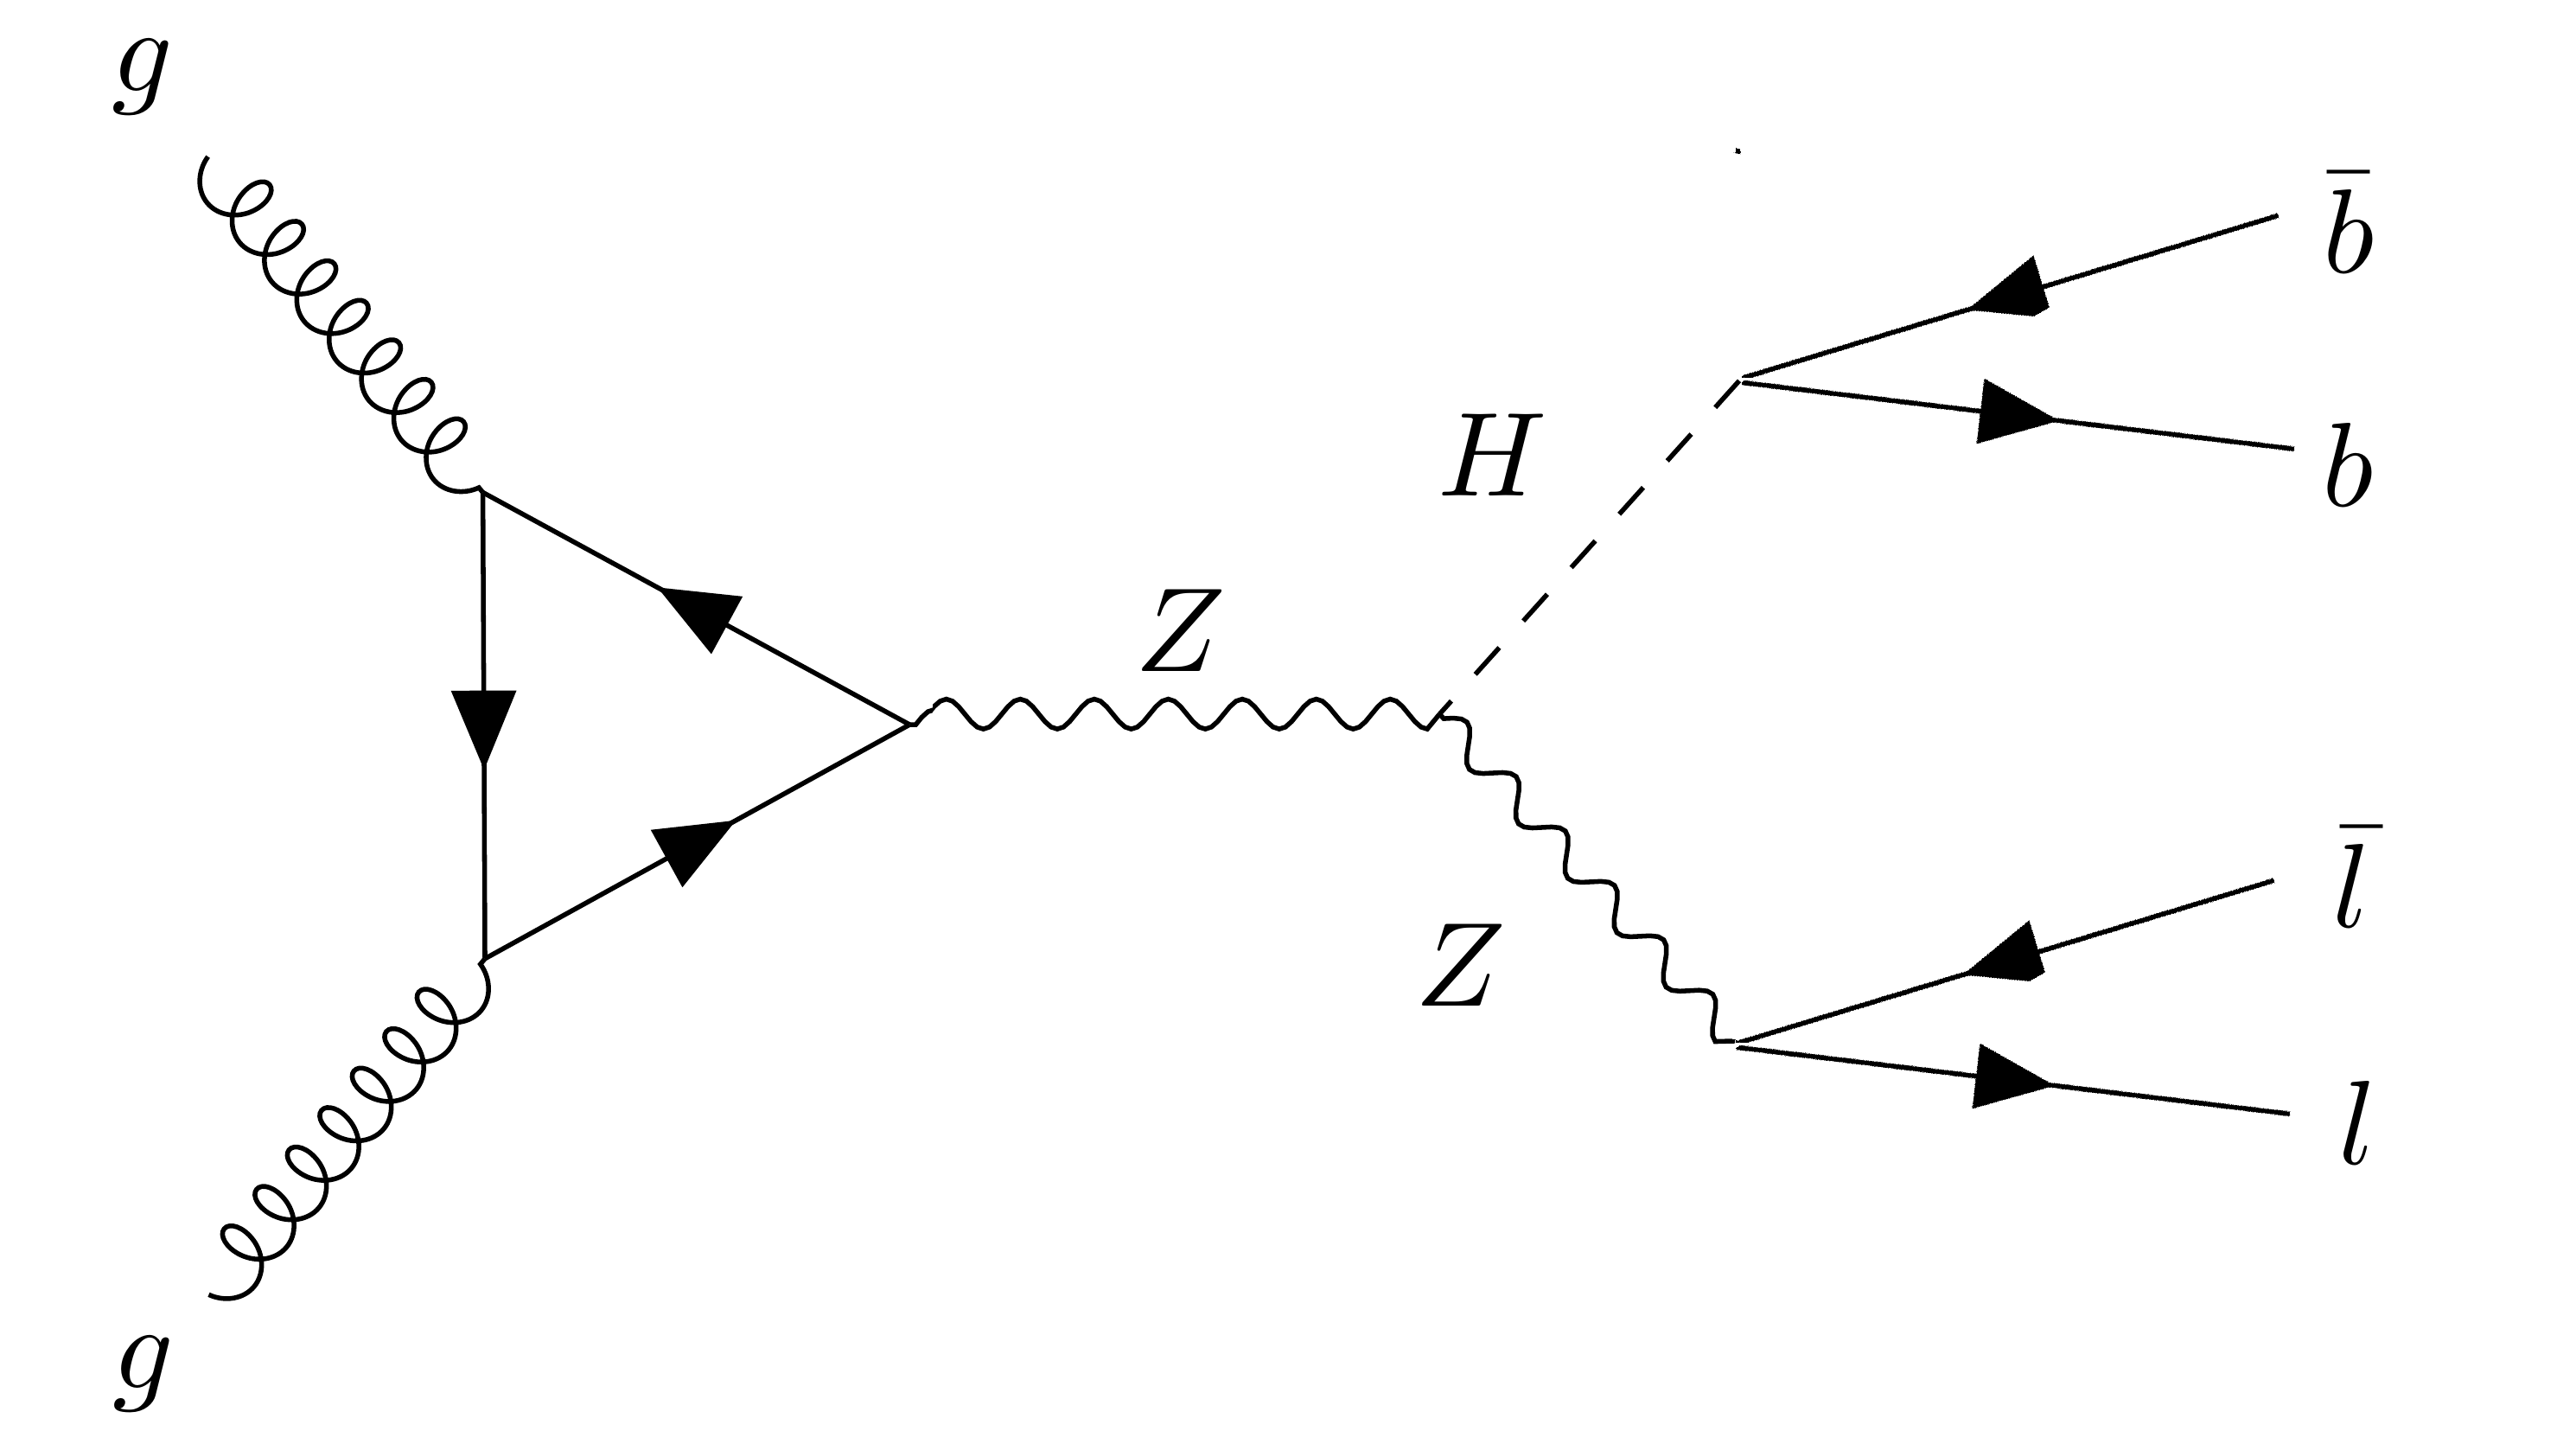
\includegraphics[width=0.4\linewidth]{figures/analysis/ggZH_triangle_bbll}&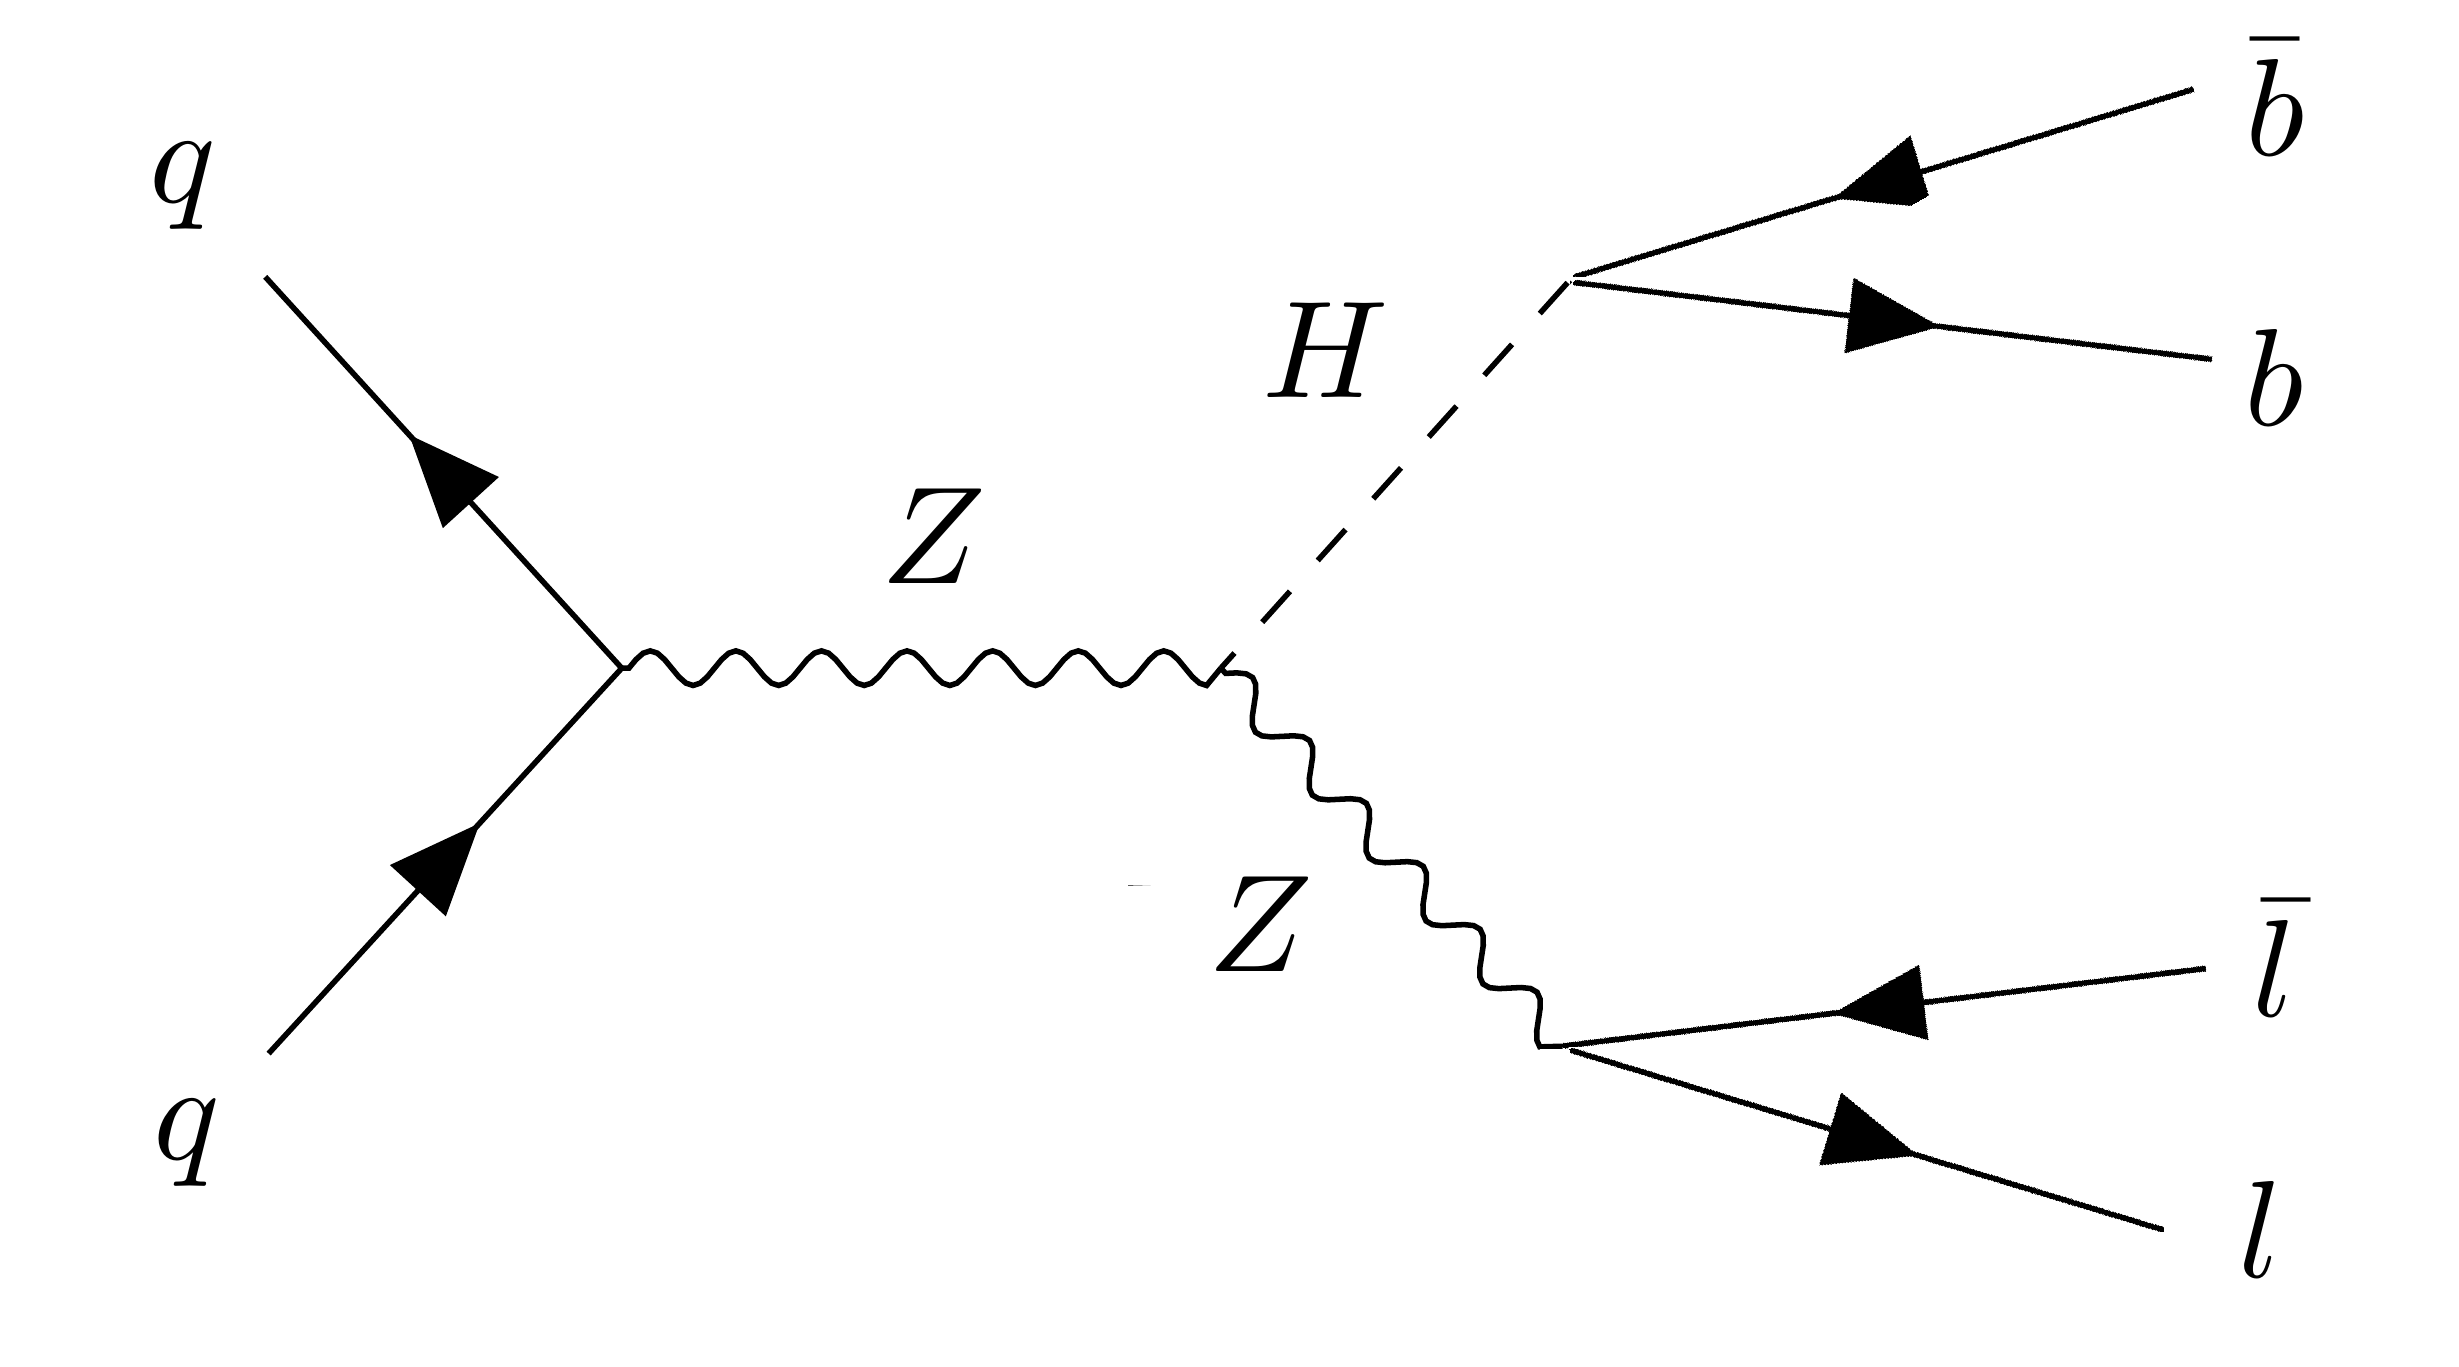
\includegraphics[width=0.4\linewidth]{figures/analysis/ZH_DY_bbll}  \\
		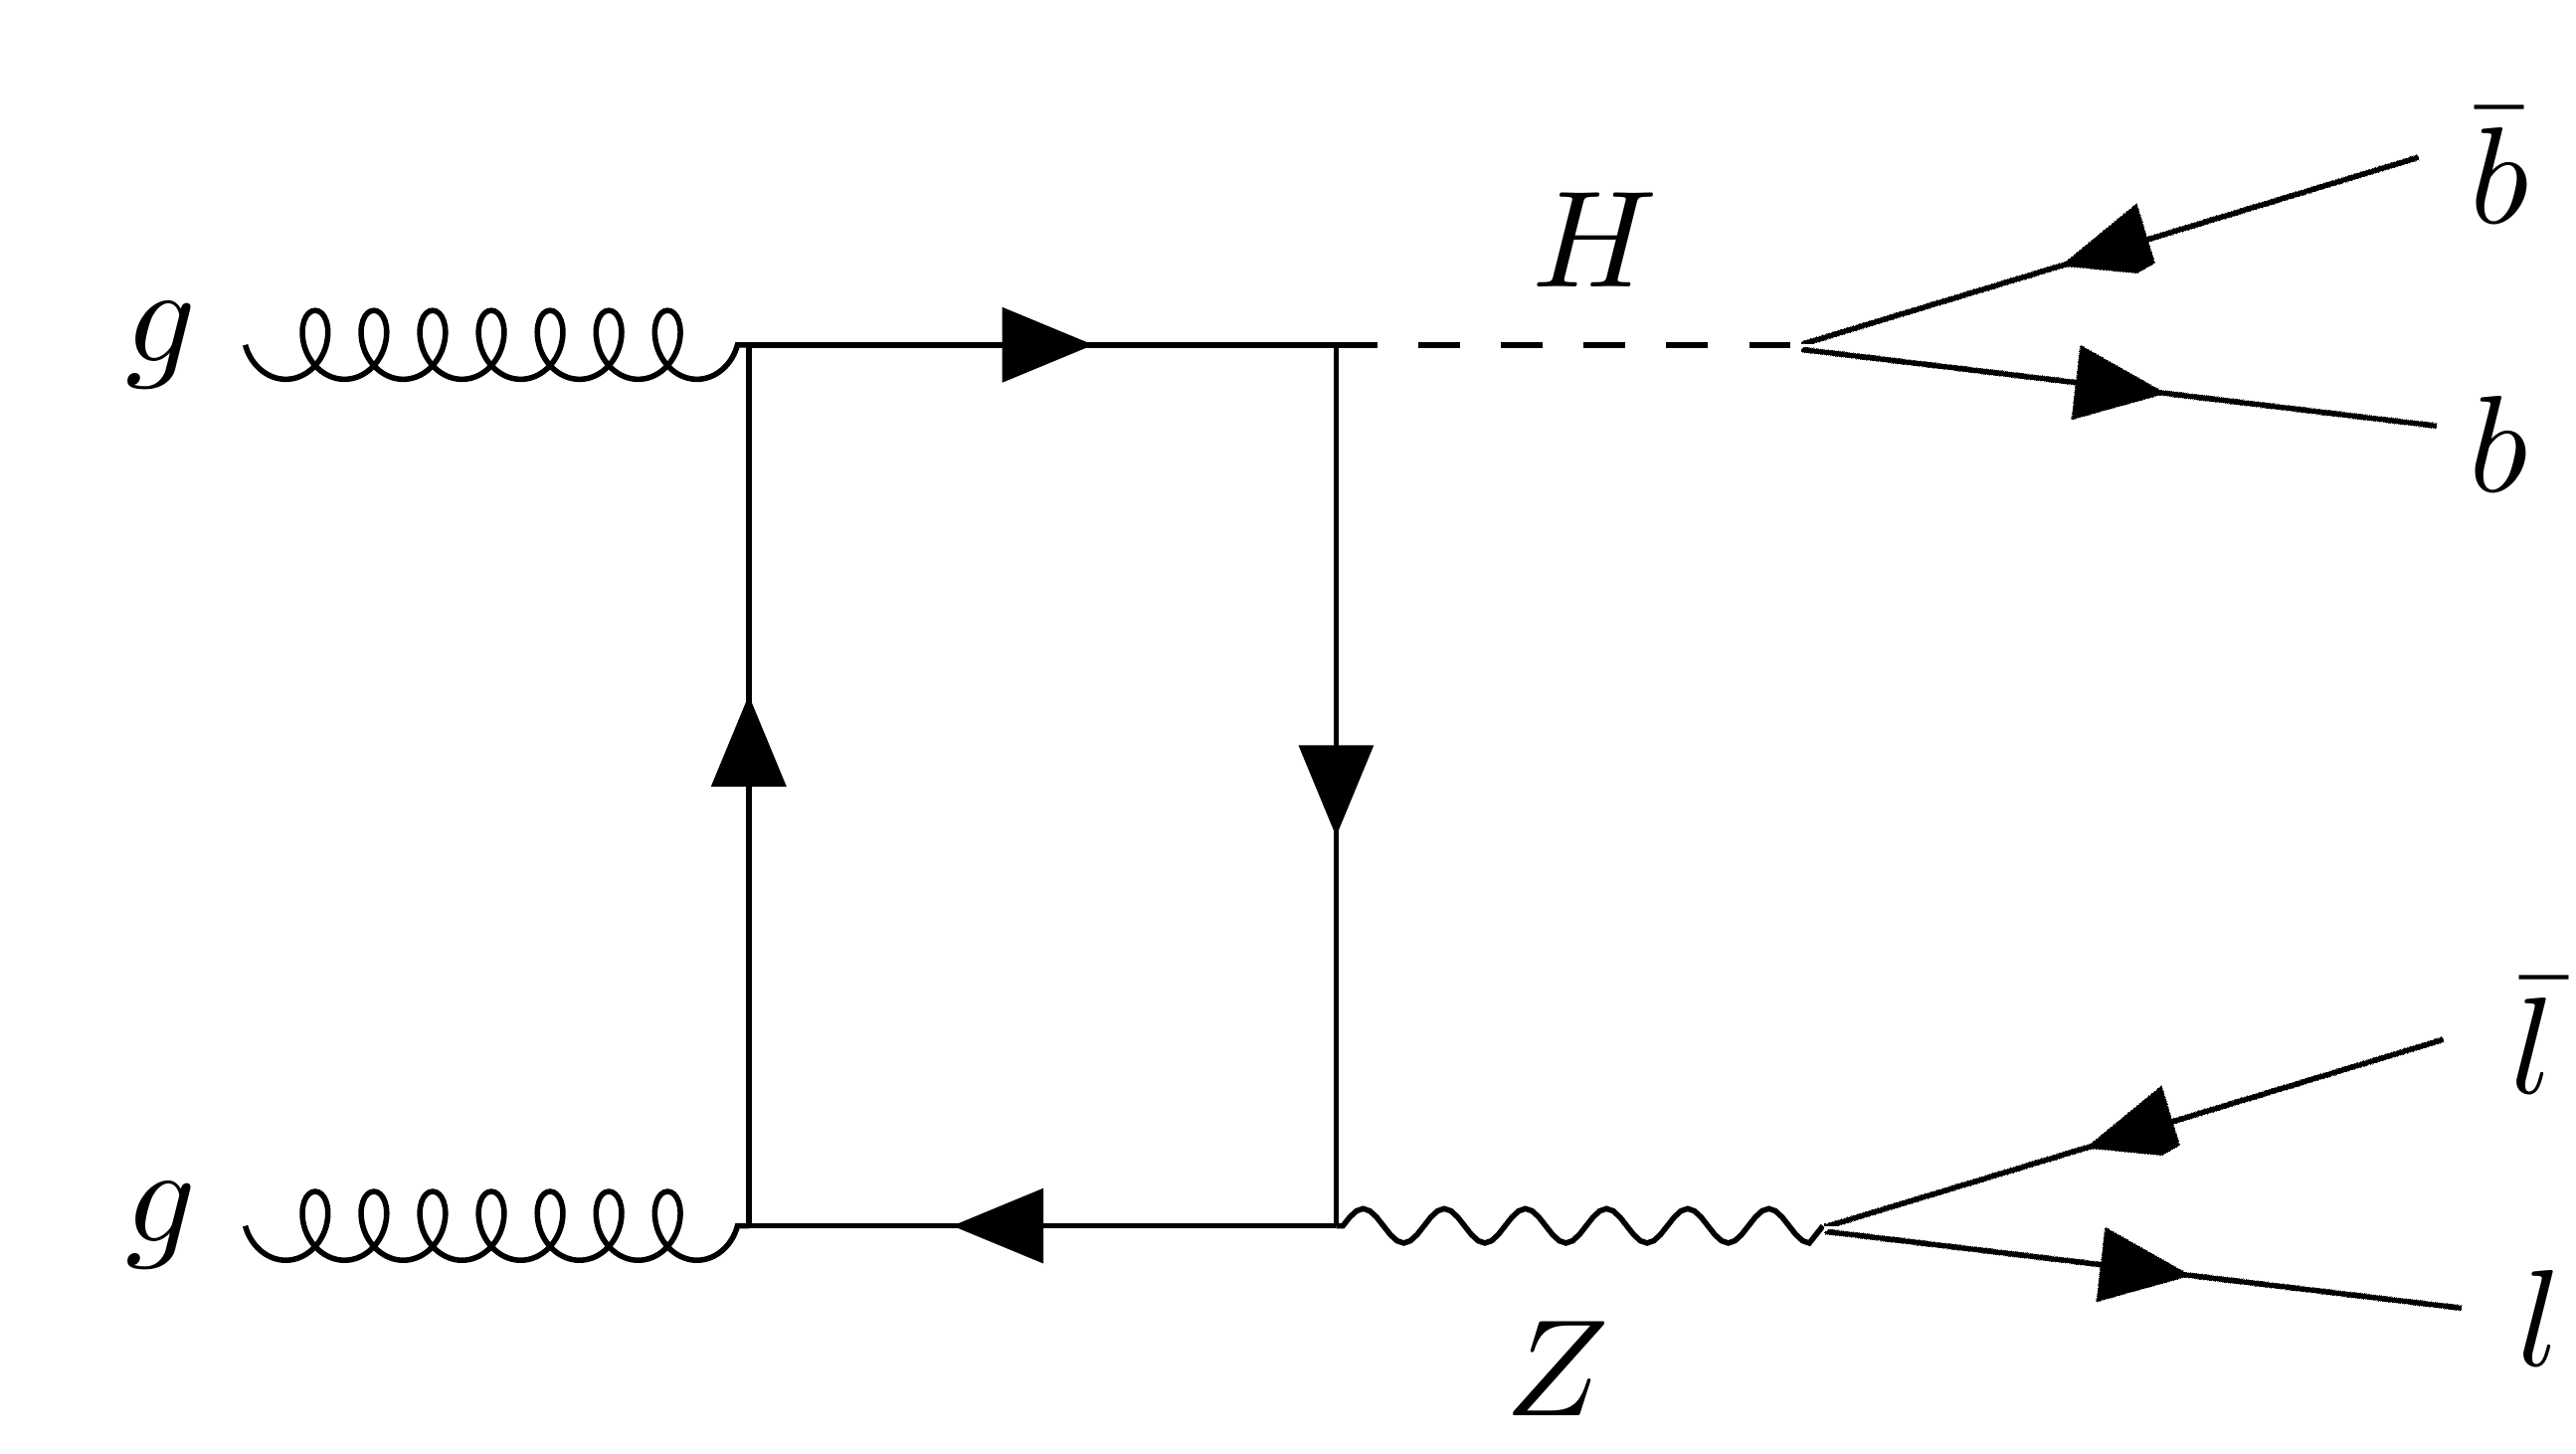
\includegraphics[width=0.4\linewidth]{figures/analysis/ggZH_box_bbll}& 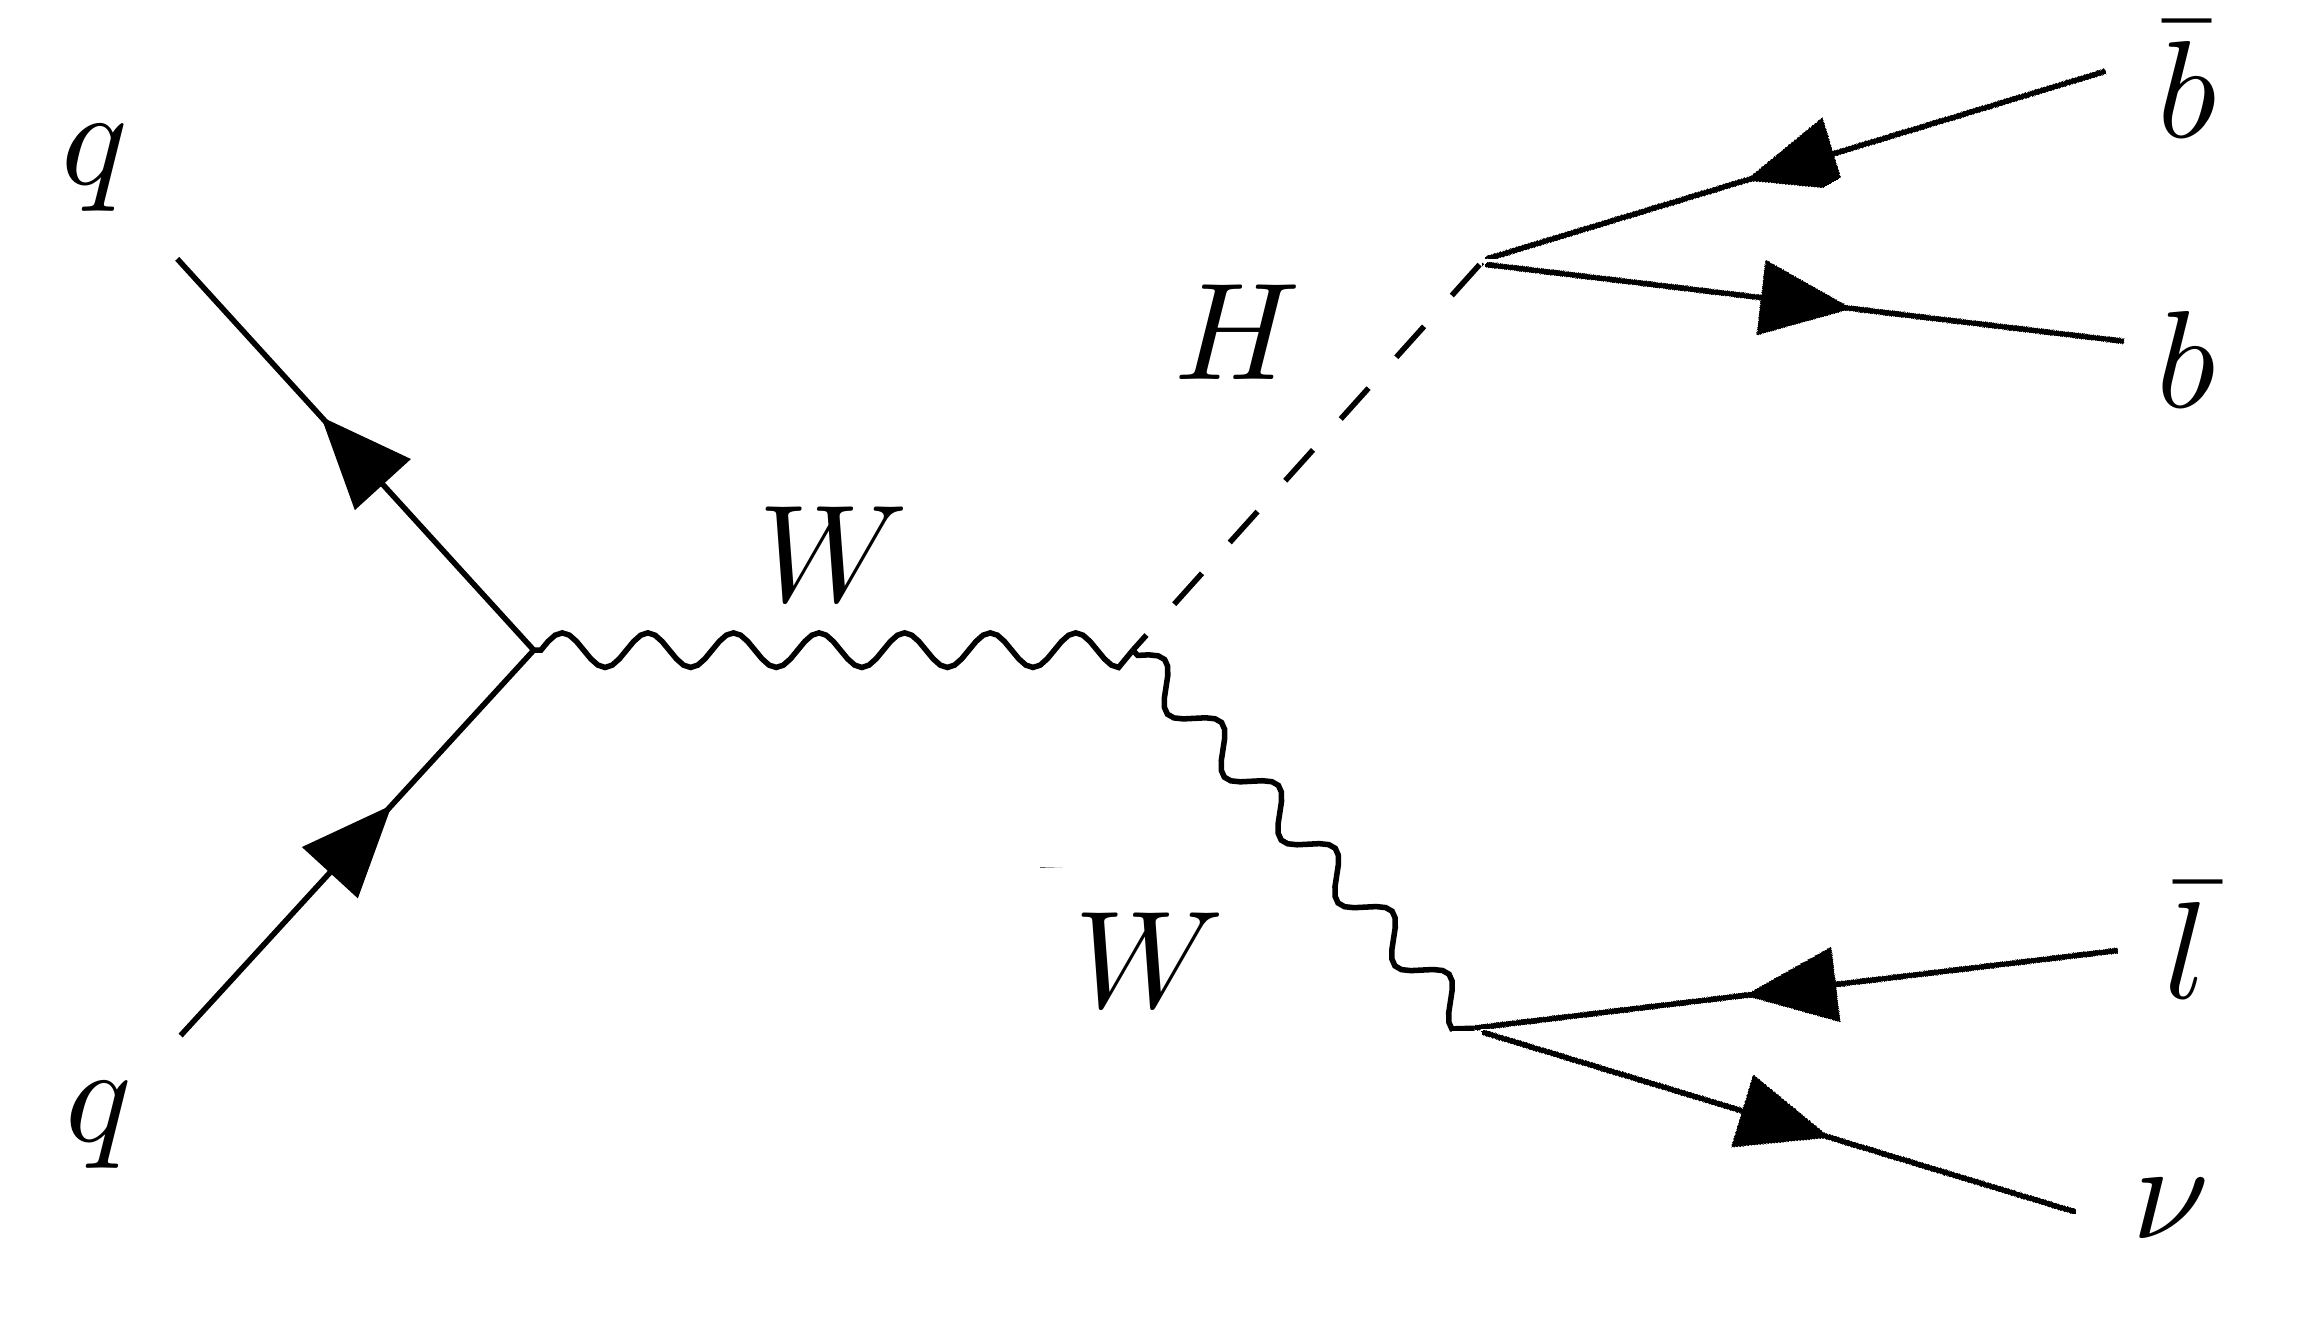
\includegraphics[width=0.4\linewidth]{figures/analysis/HWbbl} \\
	\end{tabular}
	\caption{The analysed final states of the $VH$ processes.}
	\label{fig:VH_finalstates}
\end{table}

The events are categorized through a triggering system and are assigned to one of four channels. The list of the triggers for the two and one lepton channels are listed in tab. \ref{tab:triggers}.

\begin{table}[h!]
	\centering
	\begin{tabular}{cc}
		Channel & Trigger Name \\
		\hline 
		\multirow{2}{*}{$ee$} & \texttt{Ele23\_Ele12\_CaloIdL\_TrackIdL\_IsoVL} \\
		& \texttt{Ele23\_Ele12\_CaloIdL\_TrackIdL\_IsoVL\_DZ} \\
		\hline 
		\multirow{2}{*}{$e$} & \texttt{Ele32\_WPTight\_Gsf} \\
		& \texttt{Ele32\_WPTight\_Gsf\_L1DoubleEG} \\
		\hline 
		\multirow{2}{*}{$\mu\mu$} & \texttt{Mu17\_TrkIsoVVL\_Mu8\_TrkIsoVVL\_DZ} \\
		& \texttt{Mu17\_TrkIsoVVL\_Mu8\_TrkIsoVVL\_DZ\_Mass3p8} \\
		\hline 
		\multirow{2}{*}{$\mu$} & \texttt{IsoMu24\_eta2p1} \\
		& \texttt{IsoMu27} \\
		\hline \\
	\end{tabular}
	\caption{The lepton triggers used in the analysis. For a channel, only one of the given two is used.}
	\label{tab:triggers}
\end{table}

The naming in tab. \ref{tab:triggers} indicates the phase space which the triggers select. In the two lepton channels the lepton with the higher transverse momentum (the leading lepton) is required to have $p_T > \SI{23}{\giga\electronvolt}$ and $p_T > \SI{17}{\giga\electronvolt}$ for $ee$ and $\mu\mu$, respectively; the sub-leading lepton is then required to have $p_T>\SI{12}{\giga\electronvolt}$ and $\SI{8}{\giga\electronvolt}$ for $ee$ and $\mu\mu$, respectively. In the one lepton categories, only electrons with $p_T>\SI{32}{\giga\electronvolt}$ and isolated muons with $\SI{24}{\giga\electronvolt}$ and $|\eta|<2.1$ or isolated muons with $p_T>\SI{27}{\giga\electronvolt}$ are kept.

%In addition to these selection criteria, both muon tracks have to be isolated in the $\mu\mu$ channel. For the $e$ channel, the tight working point has been selected as trigger efficiency.

\begin{table}[h!]
	\centering
	\begin{tabular}{lS[table-format=8.0]S[table-format=1.6]}
%		\toprule
		Dataset name&{N}&$\sigma/$\si{\pico\barn} \\
		\midrule
		\verb|ZH_HToBB_ZToLL_M125_13TeV_powheg_pythia8|&9530684 &0.04471\\
		\verb|ggZH_HToBB_ZToLL_M125_13TeV_powheg_herwigpp|& 199131&0.00722\\
		\midrule
		\verb|WminusH_HToBB_WToLNu_M125_13TeV_powheg_pythia8|&2382500&0.1012\\
		\verb|WplusH_HToBB_WToLNu_M125_13TeV_powheg_pythia8|&2481200&0.1595\\
%		\bottomrule
	\end{tabular}
	\caption{Simulated signal samples for the quark initiated ZH- and WH- and gluon fusion induced ZH process for 2017, with the cross section $\sigma$ of each process and the number of generated events $N$.}
%	\caption{\textcolor{red}{The signal datasets}}
	\label{tab:signal_datasets}
\end{table}

Regarding background, one distinguishes between the following processes:

\begin{itemize}
	\item[] \texttt{dy}: Drell-Yan vector boson production with hadronic initial state radiation. This process has high cross section and yields the same final state (for radiated bottom jets) as the signal. In addition, it has the same lepton signature too. The process is shown in fig. \ref{fig:dy_background}.
	\begin{figure}[h!]
		\centering
		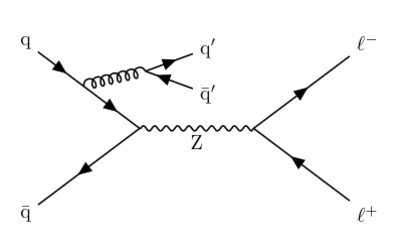
\includegraphics[width=0.4\textwidth]{figures/analysis/dy.pdf}
		\caption{The Feynman diagram for the dy background process.}
		\label{fig:dy_background}
	\end{figure}
	\item[] $\texttt{t}\bar{\texttt{t}}$: Production of top quark pairs $t\bar{t}$. These quarks decay with high probability via $t\rightarrow Wb$ and with the leptonic decay channel of the $W$, this has the same final state as the signal process and has a large background contribution. The corresponding Feynman diagram is shown in fig. \ref{fig:tt_background}.
	\begin{figure}[h!]
		\centering
		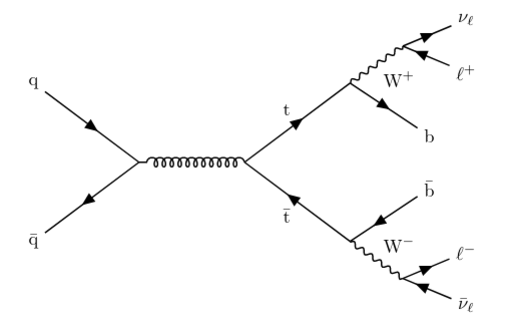
\includegraphics[width=0.5\textwidth]{figures/analysis/tt.pdf}
		\caption{The Feynman diagram for the tt background process.}
		\label{fig:tt_background}
	\end{figure}
 	\item[] $\texttt{st}$ and $\texttt{t}\bar{\texttt{t}}\texttt{V}$: Single top quark production and associated vector boson production with a $t\bar{t}$ pair. For the top quarks decaying into bottom quarks and leptonically decaying vector bosons, this yields a final state similar to the signal final state.
	\item[] \texttt{VV}, \texttt{VVV} and $\texttt{t}{\bar{\texttt{t}}}\texttt{VV}$: di- or triboson production with (or without) associated $t\bar{t}$ production. If any of these vector bosons decay hadronically while the other(s) decay leptonically, this results in a semi- or dileptonic di-bottom final state.
	\item[] $\texttt{t}\bar{\texttt{t}}\texttt{VH}$, \texttt{ggH} and \texttt{VBFH} are Higgs production channels. \texttt{wjets} are leptonically decaying jet-associated $W$ boson production. \texttt{QCD} is QCD background. \texttt{rare} are rare processes (such as four top production) with individual low contribution each.
\end{itemize}

The list of the background samples from the MC simulations are all listed in tab. \ref{tab:bkg_datasets}.

\begingroup
\footnotesize
\setlength\LTleft{-1.0cm}
\begin{longtable}[b]{llS[table-format=9.0]S[table-format=7.8]}
	\caption{List of simulated background samples for 2017 with the cross section $\sigma$ of each process and the number of generated events $N$, divided into process groups. The symbol \texttt{*} is a placeholder for \texttt{pythia8}, while \texttt{**} denotes \texttt{inclusiveDecays}. Long dataset names are split into multiple lines, denoted by an indentation. (NanoAODv7, 102X\_mc2017\_realistic\_v8-v1)}\\
	Process&Dataset name&{N}&$\sigma/$\si{\pico\barn} \\
	\midrule
	\endfirsthead
	\toprule
	Process&Dataset name&{N}&$\sigma/$\si{\pico\barn} \\
	\midrule
	\endhead
	\bottomrule
	\endfoot
	\bottomrule
	\endlastfoot
	
	\multirow{ 4}{*}{DY}&\verb|DYJetsToLL_M-10to50_TuneCP5_13TeV-madgraphMLM-*| & 79058069&18610.0\\
	&\verb|DYJetsToLL_0J_TuneCP5_13TeV-amcatnloFXFX-*| &88134822 &4843.6\\
	&\verb|DYJetsToLL_1J_TuneCP5_13TeV-amcatnloFXFX-*| & 95629091&897.8\\
	&\verb|DYJetsToLL_2J_TuneCP5_13TeV-amcatnloFXFX-*| & 54497574&335.8\\
	\midrule%t$\bar{\textrm{t}}$
	\multirow{ 3}{*}{t$\Bar{\textrm{t}}$}&\verb|TTTo2L2Nu_TuneCP5_PSweights_13TeV-powheg-*| & 68296294&88.4\\
	&\verb|TTToSemiLeptonic_TuneCP5_PSweights_13TeV-powheg-*| & 109795512&365.52\\
	&\verb|TTToHadronic_TuneCP5_PSweights_13TeV-powheg-*| &128829950&377.96\\
	\midrule
	\multirow{ 5}{*}{VV}&\verb|WWTo2L2Nu_NNPDF31_TuneCP5_PSweights_13TeV-powheg-*| & 2000000&12.2\\
	&\verb|WWTo2L2Nu_DoubleScattering_13TeV-*| & 968000&0.2232\\
	&\verb|ZZTo4L_13TeV_powheg_*| & 207798469&1.256\\
	&\verb|WZTo3LNu_TuneCP5_13TeV-amcatnloFXFX-*| & 10987679&4.43\\
	&\verb|ZGToLLG_01J_5f_TuneCP5_13TeV-amcatnloFXFX-*| & 30490034&55.59\\
	\midrule
	%&\verb|?WGToLNuG_TuneCP5_13TeV-madgraphMLM-*| &  6283083&464.800\\%aktuell auskommentiert
	%\midrule
	\multirow{ 7}{*}{ST}&\verb|ST_t-channel_top_4f_**_TuneCP5_13TeV-powhegV2-madspin-*| & 5982064&136.02\\
	&\verb|ST_t-channel_antitop_4f_**_TuneCP5_13TeV-powhegV2-madspin-*| & 3675910&80.95\\
	&\verb|ST_s-channel_4f_leptonDecays_TuneCP5_| & 9914948&3.364\\
	&\verb|     PSweights_13TeV-amcatnlo-*|\\
	&\verb|ST_tW_top_5f_**_TuneCP5_PSweights_13TeV-powheg-*| &7755138 &35.85\\
	&\verb|ST_tW_antitop_5f_**_TuneCP5_PSweights_13TeV-powheg-*| & 7745276&35.85\\
	&\verb|ST_tWll_5f_LO_TuneCP5_PSweights_13TeV-madgraph-*| & 986000&0.01096\\
    \newpage
	%\midrule
	\multirow{ 5}{*}{VVV}&\verb|WWW_4F_TuneCP5_13TeV-amcatnlo-*| & 472300&0.2086\\
	&\verb|WWZ_4F_TuneCP5_13TeV-amcatnlo-*| & 500000&0.1676\\
	&\verb|WZZ_TuneCP5_13TeV-amcatnlo-*| & 500000&0.05701\\
	&\verb|ZZZ_TuneCP5_13TeV-amcatnlo-*| & 500000&0.01473\\
	&\verb|WZG_TuneCP5_13TeV-amcatnlo-*| & 1000000&0.04345\\
	\midrule
	\multirow{ 5}{*}{t$\Bar{\textrm{t}}$V}&\verb|TTZToLL_M-1to10_TuneCP5_13TeV-amcatnlo-*| &250000 &0.0822\\
	&\verb|TTZToLLNuNu_M-10_TuneCP5_PSweights_13TeV-amcatnlo-*| &11092000 &0.2814\\
	&\verb|TTZToQQ_TuneCP5_13TeV-amcatnlo-*| &9690000 &0.5868\\
	&\verb|TTWJetsToLNu_TuneCP5_PSweights_13TeV-amcatnloFXFX-madspin-*| & 9828579&0.196\\
	&\verb|TTWJetsToQQ_TuneCP5_13TeV-amcatnloFXFX-madspin-*| &811306 &0.4049\\
	\midrule
	\multirow{ 1}{*}{t$\Bar{\textrm{t}}$VV}&\verb|TTWW_TuneCP5_13TeV-madgraph-*| & 1162000&0.006981\\
	\midrule
	\multirow{ 2}{*}{t$\Bar{\textrm{t}}$VH}&\verb|TTWH_TuneCP5_13TeV-madgraph-*| & 200000&0.001582\\
	&\verb|TTZH_TuneCP5_13TeV-madgraph-*| & 200000&0.001535\\
	\midrule
	\multirow{ 9}{*}{ggH}&\verb|GluGluHToTauTau_M125_13TeV_powheg_*| &15072210 &3.0469\\
	&\verb|GluGluHToZZTo4L_M125_13TeV_powheg2_JHUGenV7011_*| &1953198&0.01297\\
	&\verb|GluGluHToZZTo2L2Q_M125_13TeV_powheg2_JHUGenV7011_*| &1992000 &0.17963\\
	&\verb|GluGluHToWWToLNuQQ_M125_NNPDF31_TuneCP5_| &465000 &4.5621\\
	&\verb|     PSweights_13TeV_powheg_JHUGen710_*|\\
	&\verb|GluGluHToWWTo2L2Nu_M125_13TeV_powheg2_JHUGenV714_*| &953600&1.1033\\
	&\verb|GluGluHToMuMu_M-125_TuneCP5_PSweights_13TeV_powheg_*| & 1983600&0.010571\\
	&\verb|GluGluHToBB_M125_13TeV_amcatnloFXFX_*| & 9358631&28.293\\
	&\verb|GluGluHToGG_M125_13TeV_amcatnloFXFX_*| & 3942252&0.11028\\
	\midrule
	\multirow{ 7}{*}{VBF}&\verb|VBFHToTauTau_M125_13TeV_powheg_*| & 2977152&0.2372\\
	&\verb|VBF_HToZZTo4L_M125_13TeV_powheg2_JHUGenV7011_*| & 2220820&0.0010099\\
	&\verb|VBFHToWWToLNuQQ_M125_NNPDF31_TuneCP5_| & 480000&0.35517\\
	&\verb|     PSweights_13TeV_powheg_JHUGen710_*|\\
	&\verb|VBFHToWWTo2L2Nu_M125_13TeV_powheg2_JHUGenV714_*| & 500000&0.085894\\
	&\verb|VBFHToMuMu_M-125_TuneCP5_PSweights_13TeV_powheg_*| & 982200&0.00082296\\
	&\verb|VBFHToBB_M-125_13TeV_powheg_*_weightfix| & 5000000&2.2026\\
	&\verb|VBFHToGG_M125_13TeV_amcatnlo_*_PSWeights| &975930 &0.0085851\\
	\midrule
	\multirow{ 8}{*}{WJets}&\verb|WJetsToLNu_HT-70To100_TuneCP5_13TeV-madgraphMLM-pythia8| & 22255124&1504.92\\
	&\verb|WJetsToLNu_HT-100To200_TuneCP5_13TeV-madgraphMLM-pythia8| &35862893&1625.08\\
	&\verb|WJetsToLNu_HT-200To400_TuneCP5_13TeV-madgraphMLM-pythia8| & 21250517&477.96\\
	&\verb|WJetsToLNu_HT-400To600_TuneCP5_13TeV-madgraphMLM-pythia8| &14313274&67.441\\
	&\verb|WJetsToLNu_HT-600To800_TuneCP5_13TeV-madgraphMLM-pythia8| & 21709087&15.096\\
	&\verb|WJetsToLNu_HT-800To1200_TuneCP5_13TeV-madgraphMLM-pythia8| & 20432728&6.3626\\
	&\verb|WJetsToLNu_HT-1200To2500_TuneCP5_13TeV-madgraphMLM-pythia8| & 20258624&1.2658\\
	&\verb|WJetsToLNu_HT-2500ToInf_TuneCP5_13TeV-madgraphMLM-pythia8| & 21495421&0.009405\\
	\midrule
	\multirow{ 5}{*}{rare}&\verb|WpWpJJ_EWK-QCD_TuneCP5_13TeV-madgraph-*| &149000 &0.04926\\
	&\verb|TTGJets_TuneCP5_13TeV-amcatnloFXFX-madspin-*| & 25290267&4.215\\
	&\verb|TGJets_leptonDecays_TuneCP5_PSweights_13TeV-amcatnlo-*| &6649547 &1.018\\
	&\verb|tZq_ll_4f_ckm_NLO_TuneCP5_PSweights_13TeV-amcatnlo-*| & 13276146&0.07358\\
	&\verb|TTTT_TuneCP5_PSweights_13TeV-amcatnlo-*| & 2273928&0.008213\\
	\midrule
	\multirow{ 8}{*}{QCD}
	&\verb|QCD_HT100to200_TuneCP5_13TeV-madgraph-*| &93231801&23590000.0\\
	&\verb|QCD_HT200to300_TuneCP5_13TeV-madgraph-*| & 59197363&1551000.0\\
	&\verb|QCD_HT300to500_TuneCP5_13TeV-madgraph-*| & 60258921&323400.0\\
	&\verb|QCD_HT500to700_TuneCP5_13TeV-madgraph-*| & 56207744&30140.0\\
	&\verb|QCD_HT700to1000_TuneCP5_13TeV-madgraph-*| & 47610552&6344.0\\
	&\verb|QCD_HT1000to1500_TuneCP5_13TeV-madgraph-*| & 33420390&1092.0\\
	&\verb|QCD_HT1500to2000_TuneCP5_13TeV-madgraph-*| & 11634434&99.76\\
	&\verb|QCD_HT2000toInf_TuneCP5_13TeV-madgraph-*| & 5941306&20.35\\
	\label{tab:bkg_datasets}	
\end{longtable}
\endgroup
\setlength\LTleft{0.0cm}

\Subsection{Analysis Setup}

In the following, the selected electron, muon and jet final state objects (reconstructed and identified by ParticleFlow) will be described in detail. First, the physics processes are simulated, followed by a detector simulation. The resulting objects undergo a final state selection, isolating phase space regions for maximizing signal sensitivity. Depending on the event signature, they are categorized and then organized into subcategories using a deep neural network, which assigns a probability score value to them. The resulting scores can then be histogrammed and measured data can then be fitted to the resulting histogram. The analysis setup has been summarized in fig. \ref{fig:analysis_workflow}.

\begin{figure}[h!]
	\centering
	\begin{tikzpicture}
		\tikzstyle{terminator} = [rectangle, draw, text centered, rounded corners, minimum height=3em]
		\tikzstyle{connector} = [draw, -latex']
		\node [terminator, fill=blue!20, text width=1.2cm] at (0,0) (start) {Monte Carlo};
		\node [terminator, fill=blue!20, text width=2cm] at (2.6,0) (detector) {Detector Simulation};
		\node [terminator, fill=blue!20, text width = 3cm] at (6.2,0) (cat) {Object selection\\Categorization};
		\node [terminator, fill=blue!20, text width = 2.5cm] at (10.2,0) (dnn) {DNN\\Subcategories};
		\node [terminator, fill=blue!20, text width = 1cm] at (13,0) (fit) {Fit};
		\path [connector] (start) -- (detector);
		\path [connector] (detector) -- (cat);
		\path [connector] (cat) -- (dnn);
		\path [connector] (dnn) -- (fit);
	\end{tikzpicture}
	\caption{Flow chart of the analysis workflow.}
	\label{fig:analysis_workflow}
\end{figure}

\Subsubsection{Final State Objects}

The muon selection criteria are listed in tab. \ref{tab:muon_selection}. For the muons, a $p_T$-cut of 15 GeV has been required. Furthermore, they ought to be identified as tight muons and have to be contained within the tracker. It is also required that their impact parameter (IP) geometry is compatible with the primary vertex (PV) too. In addition, the IP significance \texttt{sip3d} (defined as the ratio between the uncertainty of the IP and the IP itself) is also restricted to guarantee that these muons originate from the PV. The \texttt{pfRelISO04\_all} parameter cut ensures the isolation of the muons invoking a stronger constraint on their origin.

\begin{table}[h!]
	\centering
	\begin{tabular}{c}
		\hline
		\texttt{tightId} \\
		$p_T > \SI{15}{\giga\electronvolt}$ \\
		$|\eta| \leq 2.4$ \\
		$d_{xy} \leq \SI{0.05}{\centi\meter}$ \\
		$d_z \leq \SI{0.1}{\centi\meter}$ \\
		\texttt{sip3d} $\leq 8$ \\
		$\texttt{pfRelIso04\_all} \leq 0.15$  \\
		\hline \\
	\end{tabular}
	\caption{Selection criteria for muons.}
	\label{tab:muon_selection}
\end{table}

The electron selection criteria is listed in tab. \ref{tab:electron_selection}. The electrons are required to be contained in the tracker to ensure the quality of the transverse momentum reconstruction. These electrons should also originate from the primary vertex through the impact parameter (IP) cuts $d_i$. Similarly to muons, the IP significance and isolation measures are also restricted. For quality reconstruction, the maximum number of lost hits in the tracker is also limited. \texttt{MVA ID WP80} has been chosen and as identification efficiency the 80\% working point (WP80, defined on a Drell-Yan sample) has been selected.

\begin{table}[h!]
	\centering
	\begin{tabular}{c}
		\hline
		\texttt{MVA ID WP80} \\
		$p_T > \SI{15}{\giga\electronvolt} $\\
		$|\eta| \leq 2.5$ \\
		$d_{xy} \leq \SI{0.05}{\centi\meter}$ \\
		$d_z \leq \SI{0.1}{\centi\meter}$ \\
		$\texttt{pfRelIso04\_all} \leq 0.15$  \\
		sip3d $\leq 8$ \\
		$\text{lost hits} \leq 1$ \\
		\hline \\
	\end{tabular}
	\caption{Selection criteria for the electrons.}
	\label{tab:electron_selection}
\end{table}

For the jets in consideration, the selection criteria in tab. \ref{tab:jet_selection} are applied. The AK4 jets are required to carry the tight ID. In addition to that, they are restricted to the region covered by the tracker. Based on the jet selection, the flavour tracking algorithm identifies the bottom jets. For the AK4-tagging, DeepFlavour is used.

\begin{table}[h!]
	\centering
	\begin{tabular}{c}
		\hline
		\texttt{tightId} \\
		$p_T > \SI{30}{\giga\electronvolt}$ \\
		$|\eta| < 2.4$ \\
		\hline
	\end{tabular}
	\caption{Jet selection criteria applied to the AK4 jets.}
	\label{tab:jet_selection}
\end{table}

\Subsubsection{Event Selection and Categorisation}

The selected events have been categorized depending on their final state configuration. In the network analysis, only channels with two b tagged AK4 jets with one or two lepton final states have been chosen.

In the two lepton configurations, the lepton charges are required to be opposite, such that the total charge of selected objects is $Q_{tot} = 0$. In addition to that, the invariant mass defined by the dilepton system is required to be close to the $Z$ mass and only events with a maximum absolute deviation of $\SI{15}{\giga\electronvolt}$ are kept. For the one lepton channels, such selection is not possible. Additional selection with supplementary leading lepton transverse momentum $p^l_T$ and missing transverse energy $\slashed{E}_T$ cuts is performed. A summary of these selection criteria for the considered channels are listed in tab. \ref{tab:categories}.


\begin{table}[h!]
	\centering
	\begin{tabular}{ccccc}
		channel & $\mu\mu$ & $ee$ & $\mu$ & $e$ \\
		\hline \hline \\
		$p^l_T$ & $>\SI{30}{\giga\electronvolt}$ & $>\SI{25}{\giga\electronvolt}$ & $>\SI{25}{\giga\electronvolt}$ & $>\SI{35}{\giga\electronvolt}$ \\
		$n_\mu$ & 2 & 0 & 1 & 0 \\
		$n_e$ & 0 & 2 & 0 & 1 \\
		$Q_{tot}$ & 0 & 0 & -- & -- \\
		$\slashed{E}_T$ & -- & -- & \multicolumn{2}{c}{$>\SI{30}{\giga\electronvolt}$}  \\
		$m_{ll}$ & \multicolumn{2}{c}{$|m_{ll}-m_Z|\leq\SI{15}{\giga\electronvolt}$} & -- & -- \\
	\end{tabular}
	\caption{Selected categories with the additional kinematic cuts they impose. Note that there is a channel for each trigger.}
	\label{tab:categories}
\end{table}

\Subsubsection{Multi-Process Classification and Weight Application}

Following the definition of the channels, the contained events are further categorized using a deep neural network (DNN). The network assigns these events to so-called subcategories within each channel. The input variables include properties of additional physics objects, such as AK8 jets, the physics object kinematic variables, correlations among them and additional jet and particle identification values. %The complete list of input variables is shown in tab. \ref{tab:DNN_inputs}.

\begin{comment}
\begin{table}[h!]
	\centering
	\begin{tabular}{cc}
		Object & Variable \\
		\hline
		Leptons (2) & $E, p_x, p_y, p_z, q$, PDG ID \\
		AK4 jets (4) & $E, p_x, p_y, p_z$, b-tag value \\
		AK8 jets (2) & $E, p_x, p_y, p_z$, b-tag value \\
		Correlated objects & $m_{ll}, \Delta\phi_{jj}, \Delta R_{ll}$ \\
		                   & $m_{jj}, p_{T, jj}, \Delta\phi_{jj}, \Delta R_{jj}$ \\
		                   & $\min(\Delta R_{l1j1}, \Delta R_{l1j2})$ \\
		                   & $\min(\Delta R_{l2j1}, \Delta R_{l2j2}$ \\
		                   & $m_{lljj}, N_{AK4j}, p^{miss}_T$
	\end{tabular}
	\caption{The 54 inputs of the classifier DNN with object multiplicity indicated in brackets. Note that the network has been trained as a general final state classifier, so additional kinematic variables irrelevant for the dilepton and single lepton channel analysis are also used as inputs.}
	\label{tab:DNN_inputs}
\end{table}
\end{comment}

The DNN assigns a probability to each event belonging to a process group. As the sensitivity for some rarely occuring background processes is low, these are grouped together into a common process group. Hence, for the 16 processes the analysis differentiates between there are only 13 process groups, which the DNN sorts the events into. The 13 process groups are listed in tab. \ref{tab:DNN_outputs}.

The events carry a generator weight, as it would be computationally infeasible to simulate all processes proportionally to their occurrence and have to be scaled with the experiment luminosity and process cross section. The resulting weights written as

\begin{equation*}
	w_i = \frac{\mathcal{L}\sigma w^\text{gen}_i}{\sum\limits_i w^\text{gen}_i}
\end{equation*}

with luminosity $\mathcal{L}$ and cross section $\sigma$ and are then applied to the maximum DNN score distribution histogram following the classification for each event $i$.

\begin{table}[h!]
	\centering
	\begin{tabular}{cc}
		Process group & Included Processes \\
		\hline
		\texttt{ggZH} & \texttt{ggZH} \\
		\texttt{ZH\_DY} & \texttt{ZH\_DY} \\
		\texttt{WH} & \texttt{WH} \\
		\texttt{dy} & \texttt{dy} \\
		\texttt{tt} & \texttt{t}$\bar{\texttt{t}}$ \\
		\texttt{st} & \texttt{st} \\
		\texttt{ggH} & \texttt{ggH} \\
		\texttt{VBFH} & \texttt{VBFH} \\
		\texttt{wjets} & \texttt{wjets} \\
		\texttt{QCD} & \texttt{QCD} \\
		\texttt{merged\_ttVX} & \texttt{t}$\bar{\texttt{t}}$\texttt{V}, \texttt{t}$\bar{\texttt{t}}$\texttt{VV},  \texttt{t}$\bar{\texttt{t}}$\texttt{VH} \\
		\texttt{merged\_multiboson} & \texttt{VV}, \texttt{VVV} \\
	\end{tabular}
	\caption{The output nodes of the DNN corresponding to a single process group each. Note that some process groups contain multiple rare processes which are difficult to resolve.}
	\label{tab:DNN_outputs}
\end{table}

An example output of a such classification is shown for an $ee$ category and \texttt{ZH\_DY} output node in fig. \ref{fig:ZH_DY_sub}. In total, there are $13\times4 = 52$ cases for the 13 output nodes and 4 categories. On this particular plot, the strong Drell-Yan and $t\bar{t}$ background is clearly visible, with \texttt{ZH\_DY} having the highest share among the signal processes.

\begin{figure}[h!]
	\centering
	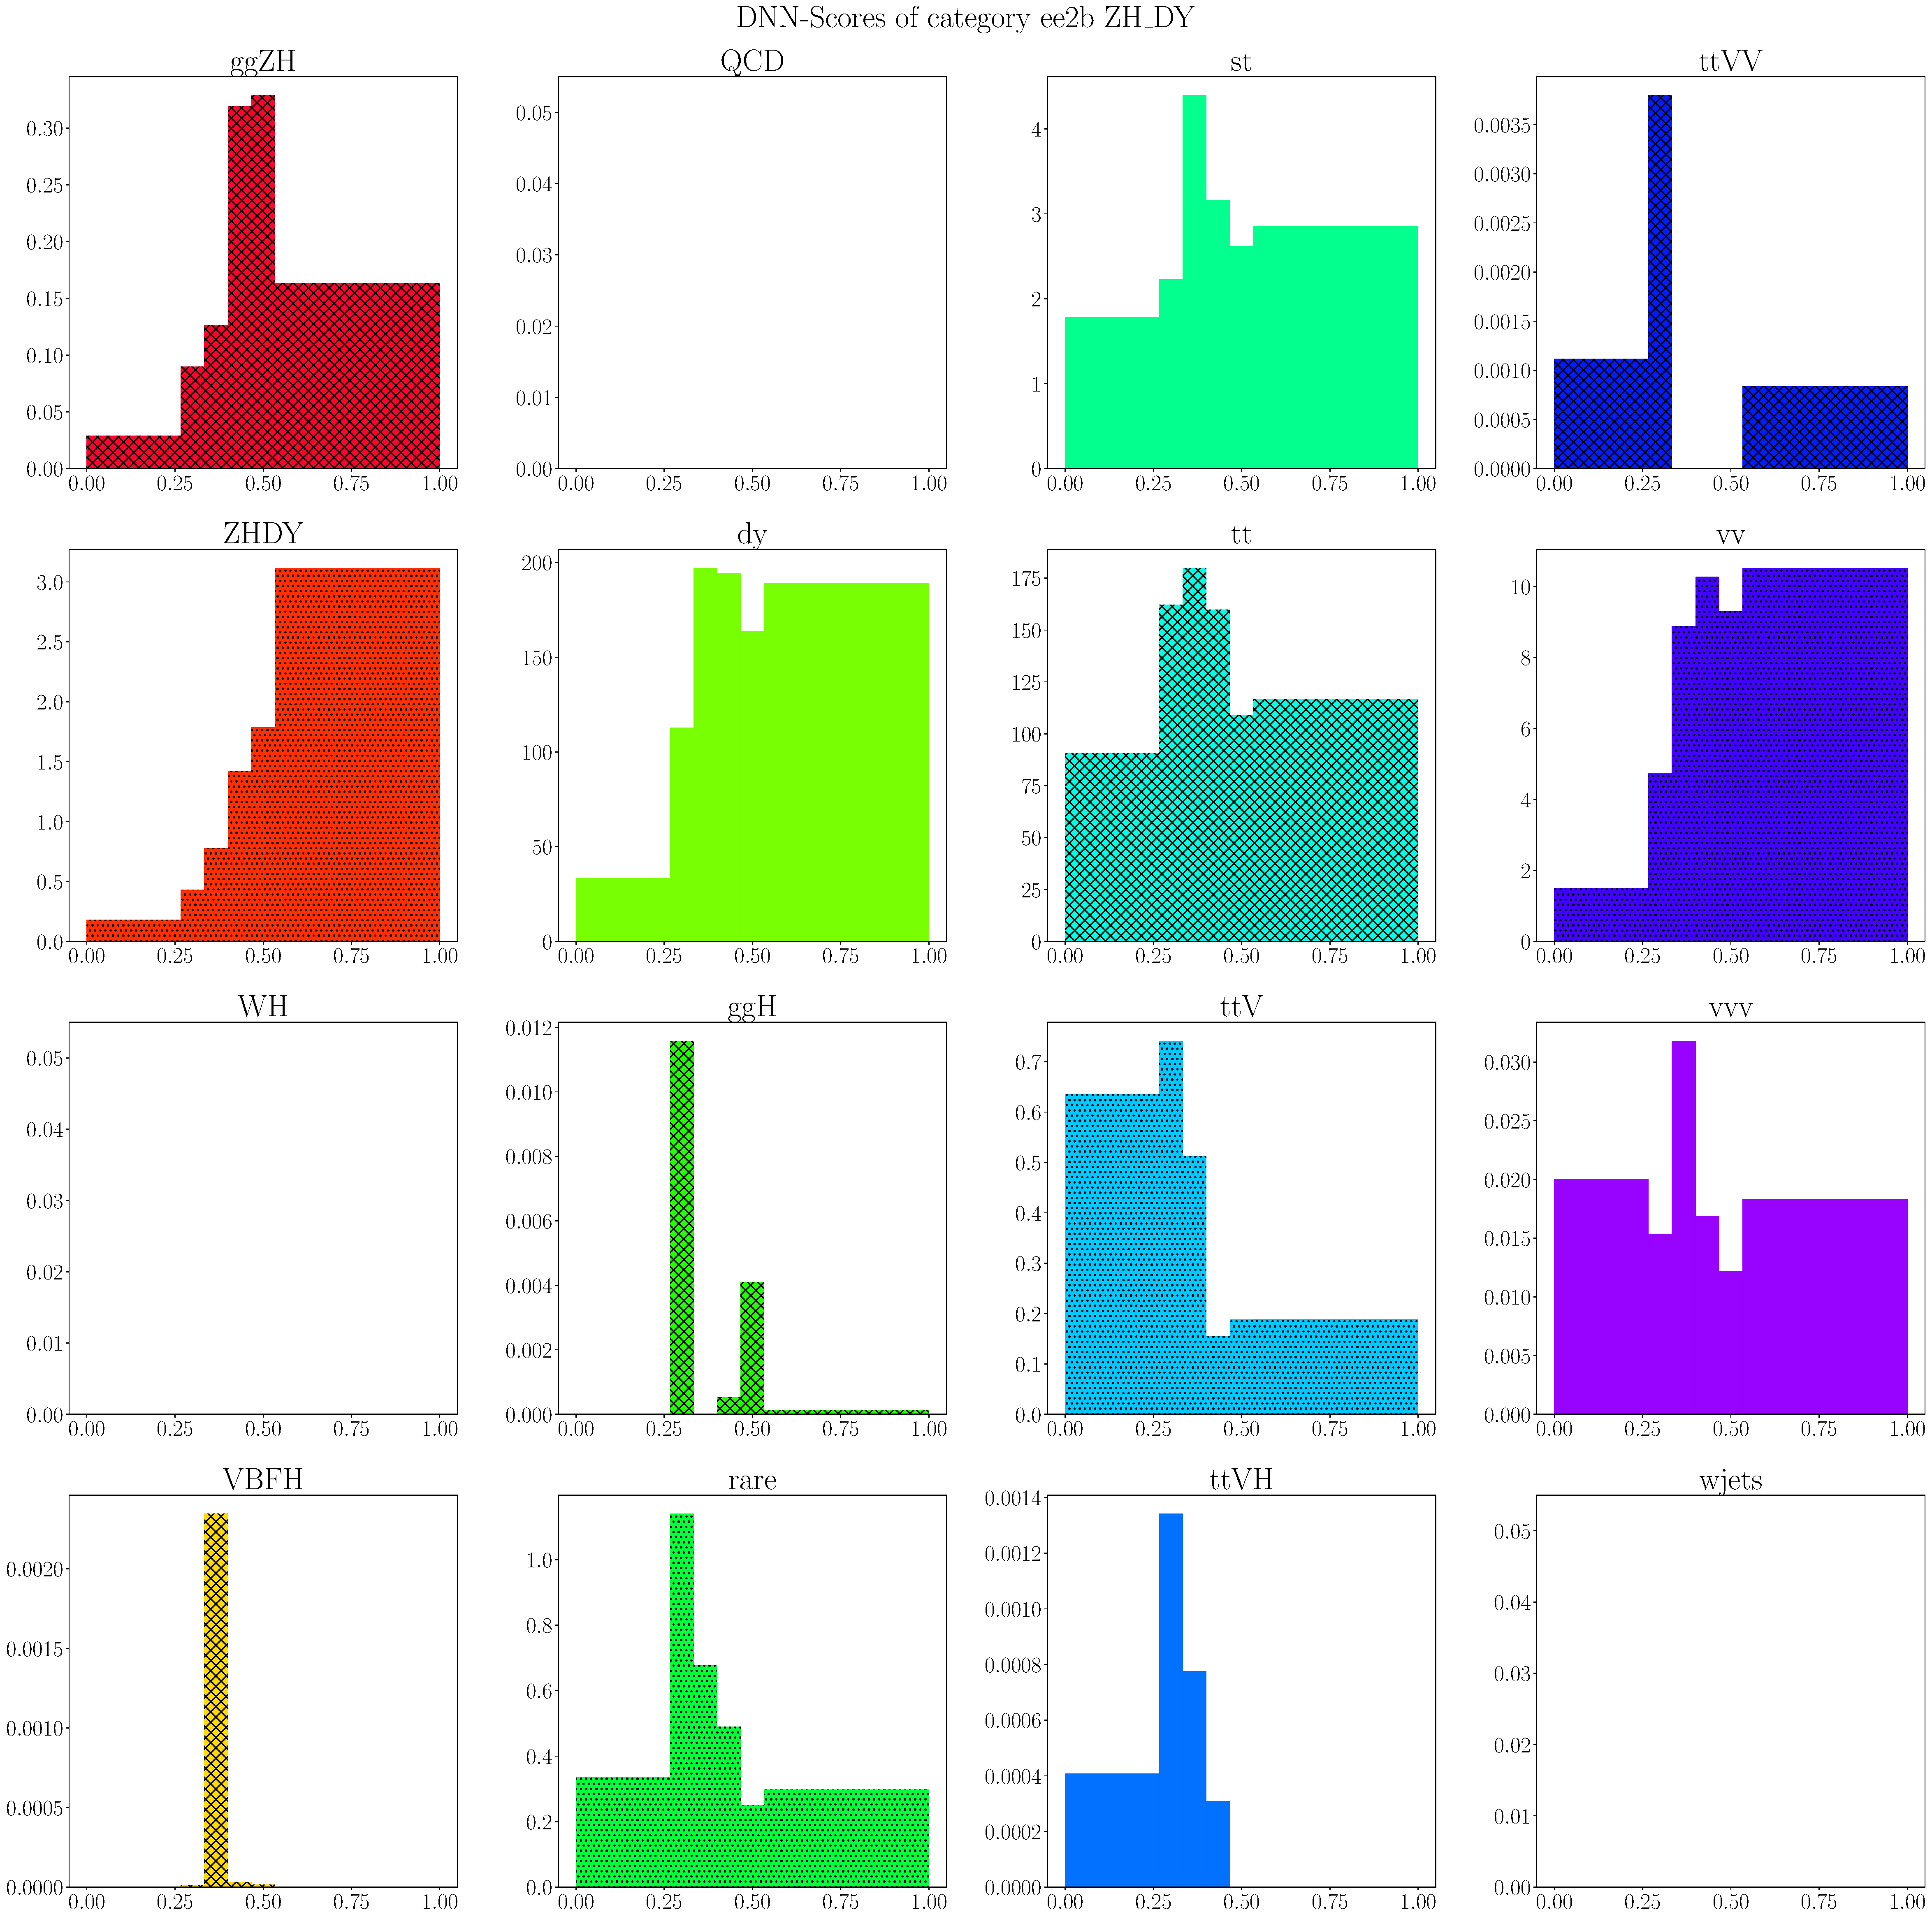
\includegraphics[width=\linewidth]{figures/analysis/ee_2b_dnn_node_ZH_DY.pdf}
	\caption{The DNN score distribution for the categorised final state objects for the \texttt{ZH\_DY} subcategory. Note the the different norming of the y axis and the high share of $t\bar{t}$, \texttt{dy} and \texttt{ZH\_DY} processes. Due to the effective categorization none of the \texttt{WH}, \texttt{QCD} and \texttt{wjets} events landed in this category. This is one of the total 52 subcategories.}
	\label{fig:ZH_DY_sub}
\end{figure}

The DNN probability score distribution of every category can be fitted to data. A such distribution for a single category is shown in fig. \ref{fig:ee_dnn_score}; for all four categories covered by this study, the resulting histogram in shown in fig. \ref{fig:conditions}. In case of a measured dataset, only the resulting bin count would be visible on which an analytical likelihood fit can be performed.

\begin{figure}[h!]
	\centering
	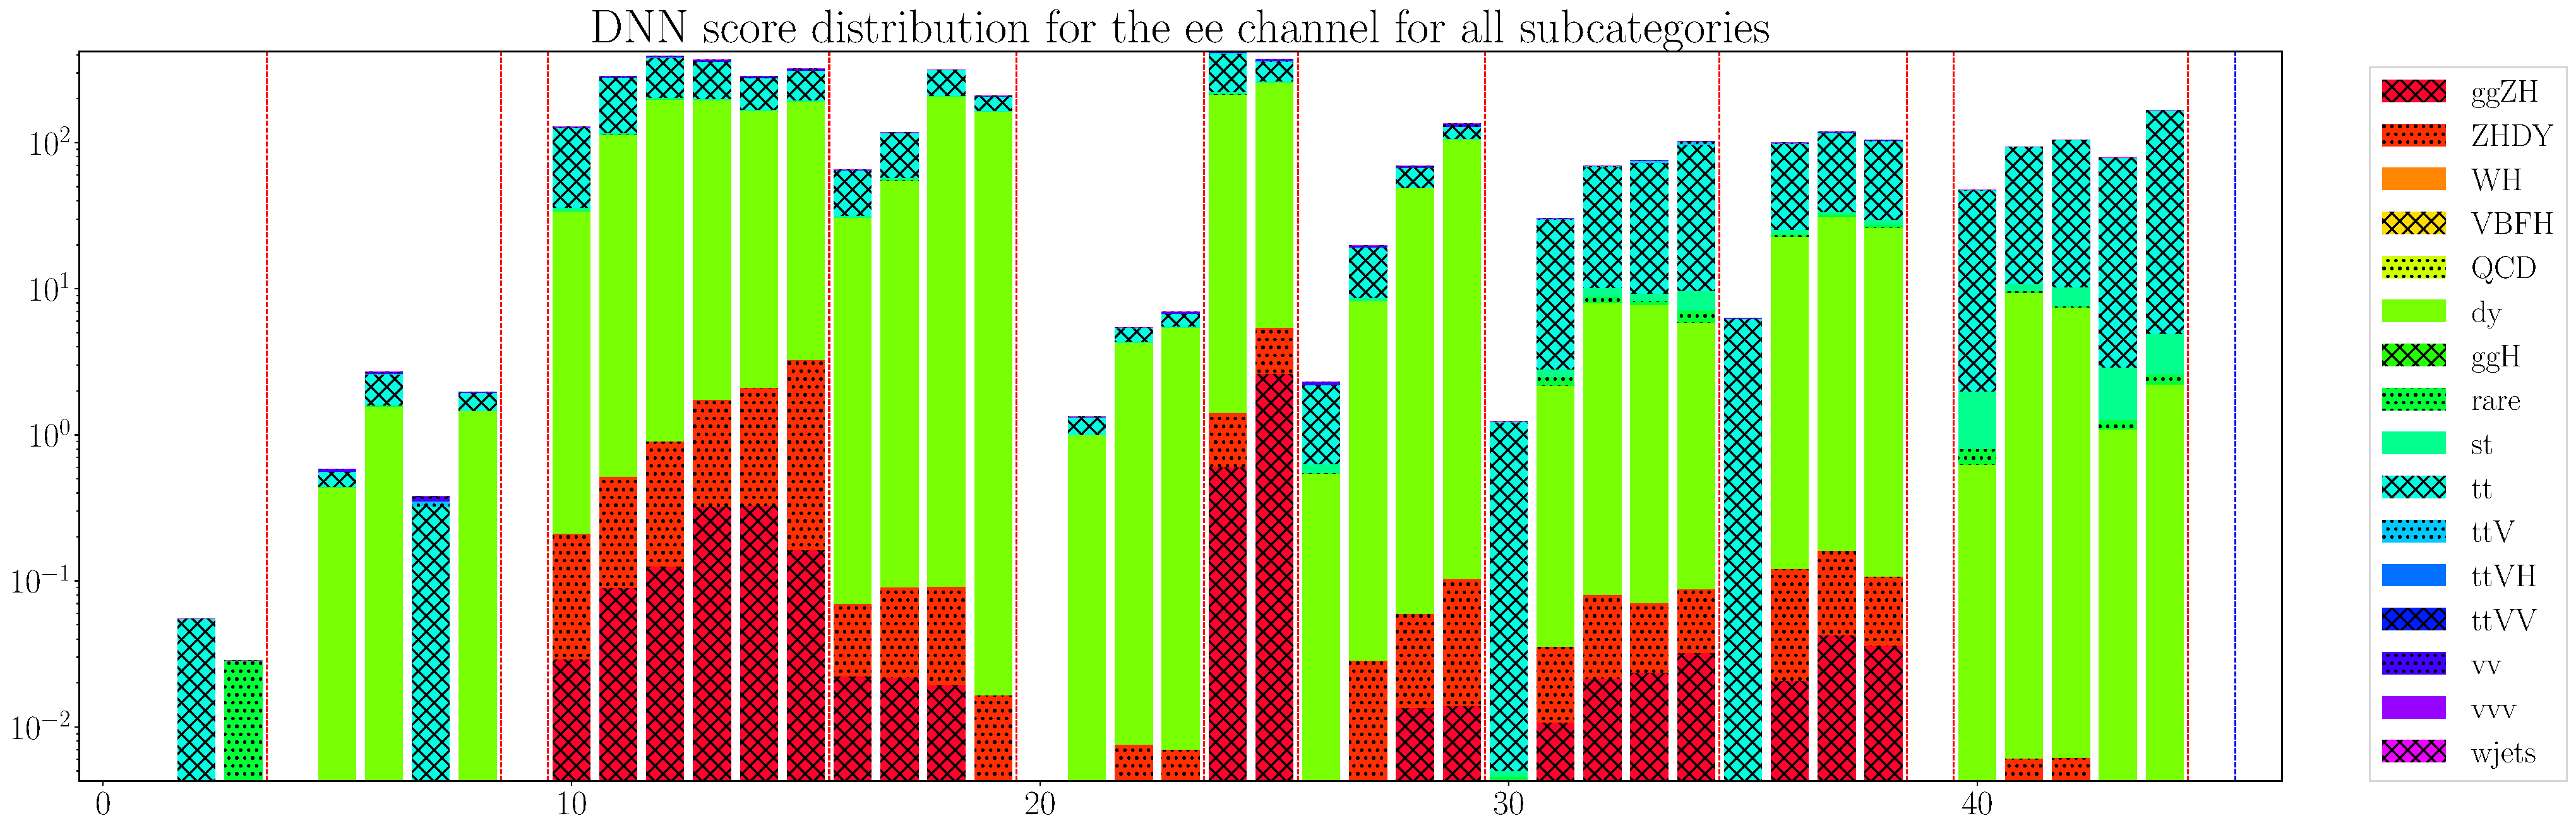
\includegraphics[width=\linewidth]{figures/analysis/cond1.pdf}
	\caption{The DNN score histogram distribution for the $ee_2b$ category and each 13 subcategory (separated in red). On the x-axis, only the bin index is shown. The fourth subcategory from the left corresponds to the above-mentioned \texttt{ZH\_DY} subcategory. The \texttt{ggZH} subcategory is the seventh from the left with the two bins. This is one of the four channels.}
	\label{fig:ee_dnn_score}
\end{figure}

\begin{figure}[h]
	\centering
	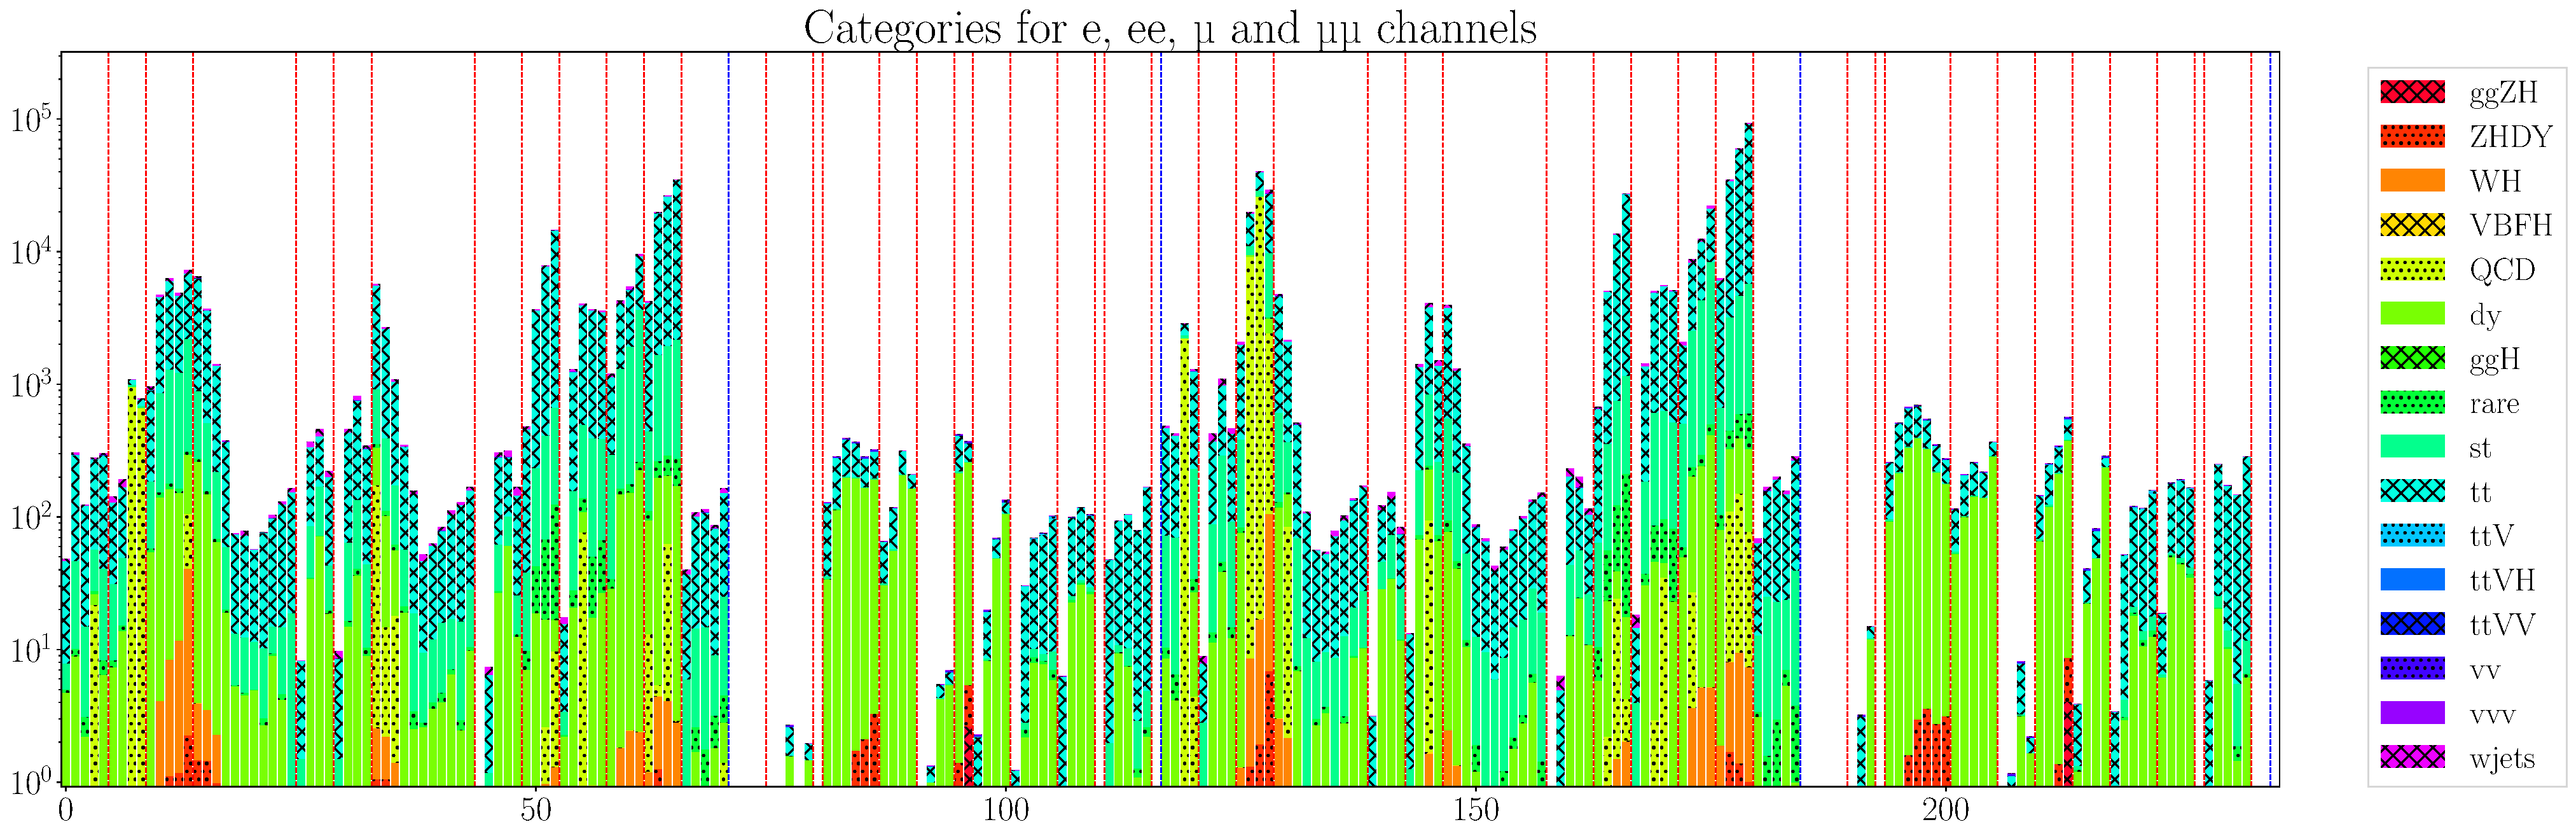
\includegraphics[width=1.1\linewidth]{figures/analysis/cond4_notOrdered.pdf}
	\caption{The distribution of the DNN scores for each subcategory (separated in red) in the one and two lepton categories in consideration (separated in blue). Note the high share of Drell-Yan, $t\bar{t}$ and QCD background events in each bin and the absence of $WH$ events in the two lepton bins. The $ee$ category is the second one from the left.}
	\label{fig:conditions}
\end{figure}

\Subsubsection{Likelihood Fits}

Using these histograms, a maximum likelihood fit can be performed to determine the signal strength parameters. For that, the likelihood function for a signal+background hypothesis is defined, which can be written as

\begin{equation*}
	\mathcal{L}(N | \left\{\mu_i\right\} , \left\{\theta_i\right\}) = \prod\limits_i \frac{(\mu_is_i(\theta)+b_i(\theta))^N}{N!}e^{-\mu_is_i(\theta) + b_i(\theta)} \prod\limits_j p(\tilde{\theta}_j | \theta_j)
\end{equation*}

The binwise signal and background contributions $s_i$ and $b_i$ depend on the uncertainty-modelling nuisance parameter $\theta$ and are Poisson-distributed; the nuisance parameters follow the probability distribution $p(\tilde{\theta} | \theta)$. This likelihood function is fitted to the histogram and encodes the variations of the background processes within the uncertainties.

In this thesis, these signal strength modifier parameters will inferred using a conditional invertible neural network and will be compared to their maximum likelihood counterpart.